\section{Introducci\'on y objetivos}
Hacia fines del siglo XIX y principios del siglo XX (\alert{revisar}), con el prop'osito de estudiar la estructura interna de una pieza musical, 
Heinrich Schenker elabor'o un m'etodo de an'alisis musical conocido como \texttt{an'alisis schenkeriano}.
Esta estructura es descripta por el autor en t'erminos de \texttt{reducciones}. Una reducci'on permite especificar que una cierta nota dentro de un grupo es la fundamental, 
y que todo el resto es una \texttt{elaboraci'on} de esta. Dado que esta relaci'on de reducci'on/elaboraci'on se puede aplicar recursivamente, naturalmente emerge una relaci'on 
jer'arquica entre las notas de una pieza musical.  En esta jerarqu'ia, el nivel m'as bajo es lo que se encuentra escrito en la partitura, y a medida que se sube de nivel se 
encuentra la misma pieza musical, pero carente de elaboraciones. A continuaci'on se excibe un ejemplo de dicho an'alisis:


\begin{figure}[h]
\begin{center}
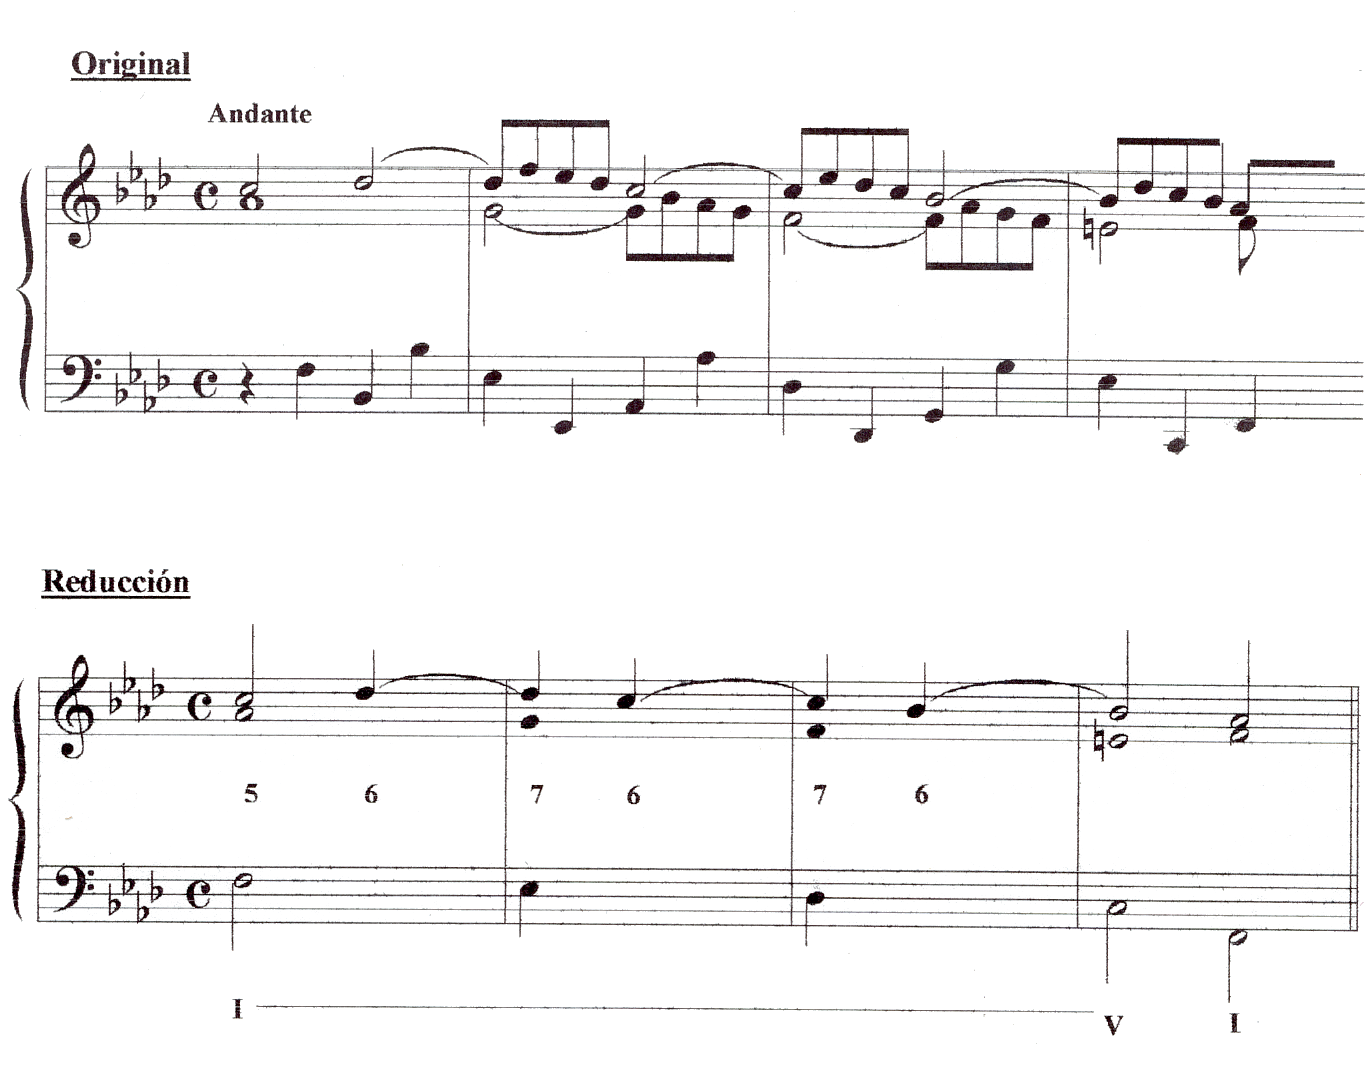
\includegraphics[width=12cm]{images/schenkerian_example.png}
\newline \alert{poner una imagen mas copada}
\end{center}
\end{figure}

En esta figura, los sucesivos pentagramas muestran relaciones de reducci'on, as'i simplificando el tema con el objeto de llevarlo a una representaci'on mas concreta.

El parecido de este tipo de relaciones con las relaci'ones utilizadas por Noam Chomsky para analizar el lenguaje natural es notable. 
Si bien en la teor'ia de Chomsky las relaciones son relaciones del tipo ``es un'', y en la teor'ia de Schenker son del tipo ``es una elaboraci'on de'', 
estas se enmarcan matem'aticamente en el mismo lugar.  

En 1983, el m'usico Fred Lerdahl y el ling\"uista Ray Jackendoff publicaron el libro 
\texttt{A Generative Theory of Tonal Music}(GTTM) donde proponen una gram'atica para analizar la m'usica t'erminos parecidos a los de Schenker. 
Lo hace interesante a este trabajo es el fundamento que se le da a la elecci'on de las reglas de la gram'atica, puesto que analizan la teor'ia 
schenkeriana en t'erminos cognitivos.  

El objetivo del trabajo de Lerdahl y Jackendoff es principalmente tener un modelo que sea capaz de describir el proceso mediante el cual se estructura la percepci'on de la m'usica. 
Este modelo consiste en una serie de reglas de preferencia. Cada regla tiene asociado un predicado booleano $P$ y un valor de preferencia $v$, 
de modo que si el predicado booleano es verdadero, entonces aportan $v$ unidades a la preferencia de una cierta acci'on interpretativa. Para ejemplificar, a continuaci'on se cita
una regla de preferencia de los autores. Esta regla es una de las reglas asociadas a lo que los autores llaman agrupamiento, que b'asicamente consiste en agrupar notas que tienen
significancia de frase\footnote{M'as adelante se explicar'a esto con mayor detalle}.
\newline

\begin{center}
\texttt{GPR 1} Evite fuertemente grupos que contengan solamente un evento.
\end{center}

En este caso, el predicado booleano es aquel que es verdadero solamente con grupos de cardinalidad uno, y el valor de preferencia es fuertemente negativo a la acci'on interpretativa
de decidir que el grupo en cuesti'on debe contener 'unicamente al evento que contiene. Como esta, los autores exiben un gran conjunto de reglas que luego validan experimentalmente. 

Si bien un modelo de este tipo es generativo en el sentido de que podr'ia ser utilizado por una computadora tanto para analizar una pieza musical como para 
\texttt{generar} una nueva, es importante notar que este no es su objetivo. 
Puede verse claramente como la regla \emph{GPR 1} si bien es suficientemente rigurosa como para luego poder corroborarla emp'iricamente, no lo es como para construir un 
programa que haga un an'alisis utilizando esta regla: es necesario determinar el valor de preferencia y aprender las relaci'ones entre los distintos valores de preferencia para luego 
tomar una desici'on.  

De esta forma se discrimina entre \texttt{modelos generativos}, que son aquellos que eventualmente podr'ian utilizarse para generar aquello que explican, y 
\texttt{modelos de 'indole generativo} que fueron hechos con el objeto de generar aquello que explican.  El hecho de que sea necesario definir expl'icitamente los valores de preferencias
sumado a que este modelo no es de 'indole generativo plantea el interrogante de si realmente este enfoque es el adecuado para para modelar la cognici'on musical con aprendizaje 
autom'atico. 

De este modo, el objetivo de este trabajo es utilizar el conocimiento generado por trabajos como el de Lerdahl y Jackendoff como medio para establecer propiedades que un modelo de 
'indole generarivo deber'ia cumplir. Teniendo estas propiedades, luego es posible construir un modelo desvinculado con la idea de gram'atica, pero que respete 
ciertos criterios fundamentales. Si se logra conseguir un modelo de estas caracter'isticas se podr'an validar emp'iricamente los criterios en base a los que el modelo fue construido 
(y por lo tanto las teor'ias cognitivas motivaron los criterios) a trav'es de analizar las piezas musicales generadas por el modelo.

Para poder avanzar en pos del objetivo recien planteado, es necesario primero sentar un vocabulario para luego poder contextualizarlo. De esta forma, las siguientes dos
secci'ones hablaran sobre background. Luego se har'a un breve resumen sobre el estado del arte en este tema, para luego abordar el trabajo en concreto de esta tesis.

